\documentclass[conference]{IEEEtran}
\usepackage[utf8]{inputenc}
\usepackage[T1]{fontenc}
\usepackage{amsmath,amssymb}
\usepackage{graphicx}
\usepackage{booktabs}
\usepackage{hyperref}
\usepackage{xcolor}
\usepackage{tikz}
\usetikzlibrary{shapes.geometric, arrows.meta, positioning, fit, backgrounds}
\usepackage{multirow}
\usepackage{url}
\hypersetup{
    colorlinks=true,
    linkcolor=blue,
    citecolor=blue,
    urlcolor=blue
}
\begin{document}
\title{Context Is All You Need:\\Evolutive Agentic Intelligence through\\Context-Time Training (CTT)}
\author{
\IEEEauthorblockN{Mauricio Perera}
\IEEEauthorblockA{Automators.work / Rckflr\\
Quer\'etaro, Mexico\\
mauricio.perera@gmail.com}
}
\maketitle
\begin{abstract}
Traditional approaches to enhancing Large Language Model (LLM) performance, such as supervised fine-tuning (SFT), often incur prohibitive computational costs, introduce data obsolescence, and suffer from irreversible weight updates. We present \textbf{Context-Time Training (CTT)}, a novel machine learning paradigm that shifts the focus from model-centric training to agent-centric evolution. Under CTT, the underlying LLM remains a frozen, static reasoning engine, while the agent's intelligence is developed through a continuous cycle of experience accumulation, automated mining, and multi-vector consolidation.
We implement this framework in \textbf{RepoMemory v2}, a Git-inspired persistent memory system that utilizes content-addressable storage and immutable commit chains to provide a transparent and versioned audit trail of an agent's knowledge. Our architecture employs a hybrid retrieval engine---combining lexical TF-IDF with a 3-level Matryoshka neural pyramid---to optimize context injection within the transformer's attention mechanism.
Empirical benchmarks demonstrate that CTT significantly compensates for model scale: a 0.6B parameter model augmented with CTT consistently outperforms 20B parameter models without memory, achieving an average precision increase of \textbf{202\%} across technical and support domains. Furthermore, we introduce the \emph{Correction Boost} mechanism, which applies a 2.0$\times$ scoring multiplier to corrective memories, effectively resolving the ``stale fact'' problem inherent in standard RAG systems. Our results suggest that for the next generation of autonomous agents, sophisticated context management is not just a supplement to model weights---\emph{Context Is All You Need}.
\end{abstract}
\begin{IEEEkeywords}
Context-Time Training, Agentic Memory, Large Language Models, RepoMemory, Context Injection, Machine Learning Paradigms.
\end{IEEEkeywords}
% ============================================================
\section{Introduction}
The rapid advancement of Large Language Models (LLMs) has democratized access to high-capacity reasoning engines. However, the creation of persistent autonomous agents faces a fundamental obstacle: the inherent ``amnesia'' of static models. Traditionally, the industry has addressed the injection of new knowledge or the alteration of behaviors through Supervised Fine-Tuning (SFT). Nevertheless, SFT presents critical limitations: high computational costs, susceptibility to catastrophic forgetting~\cite{kirkpatrick2017overcoming}, obsolescence of data baked into model weights, and near-zero reversibility when erroneous information is learned.
As an alternative, Retrieval-Augmented Generation (RAG)~\cite{lewis2020retrieval} has partially mitigated these problems by externalizing knowledge. However, conventional RAG is passive; it retrieves static documents but does not allow the agent to \emph{learn}, \emph{consolidate} experience, or \emph{proactively correct} its own interactive biases over time.
In this paper, we present \textbf{Context-Time Training (CTT)}, a paradigm shift positing that the evolution of an intelligent agent does not require the mutation of the underlying neural networks. Under the CTT framework, the LLM is treated as immutable cognitive ``hardware,'' while the agent is trained by accumulating a dynamic and versioned knowledge base. To instantiate this framework, we introduce \textbf{RepoMemory v2}, a Git-inspired persistent memory system. Through this system, we demonstrate that algorithmic and hierarchical context management allows small language models (sub-1B parameters) to outperform massive architectures (20B parameters), empirically proving that, for long-term agentic cognition, \emph{context is all you need}.
% ============================================================
\section{Related Work}
\subsection{Retrieval-Augmented Generation}
RAG~\cite{lewis2020retrieval} pioneered the externalization of knowledge by combining a neural retriever with a generative model. Subsequent work has refined retrieval pipelines through dense passage retrieval~\cite{karpukhin2020dense}, iterative retrieval, and modular architectures~\cite{gao2023retrieval}. However, standard RAG systems treat the knowledge base as a static corpus: documents are indexed once and retrieved passively. They lack mechanisms for the agent to autonomously curate, consolidate, or version-control its own knowledge, making them fundamentally unsuitable for long-term agentic evolution.
\subsection{Memory-Augmented LLM Agents}
MemGPT~\cite{packer2023memgpt} introduced an OS-inspired virtual context management system with a two-tier memory hierarchy (main context and external storage), using function calls to page data in and out of the LLM's context window. While MemGPT demonstrated the value of hierarchical memory, it relies on the LLM itself to manage memory operations, introducing latency and potential cascading errors in memory decisions.
A-Mem~\cite{xu2025amem} proposed an agentic memory system inspired by the Zettelkasten method, where memories are dynamically organized through linking and indexing. This approach achieves adaptive organization but does not provide versioning, auditability, or correction mechanisms for erroneous memories.
Generative Agents~\cite{park2023generative} demonstrated emergent social behaviors in multi-agent environments by equipping LLM agents with memory streams, reflection, and planning modules. Their memory architecture stores observations as natural language records with timestamps, but lacks structured consolidation or deduplication mechanisms.
\subsection{Learning Without Weight Updates}
Reflexion~\cite{shinn2023reflexion} shares the closest philosophical alignment with CTT: it reinforces language agents through linguistic feedback rather than gradient updates, maintaining reflective text in an episodic memory buffer. However, Reflexion is task-episodic (reflections are scoped to individual task attempts) and does not address persistent, cross-session knowledge accumulation or semantic conflict resolution.
In-Context Learning (ICL)~\cite{brown2020language} demonstrated that LLMs can acquire new capabilities from examples provided in the prompt, without weight modification. CTT extends this principle from single-turn demonstrations to a continuous, multi-session learning framework with structured memory management.
\subsection{Positioning of CTT}
Table~\ref{tab:comparison} summarizes how CTT and RepoMemory v2 differ from prior systems. The key differentiators are: (1)~immutable version control with full audit trail, (2)~a formalized five-phase learning loop operating across sessions, (3)~the Correction Boost mechanism for resolving stale facts, and (4)~empirical validation showing sub-1B models outperforming 20B models.
\begin{table}[t]
\centering
\caption{Comparison of agentic memory systems.}
\label{tab:comparison}
\footnotesize
\setlength{\tabcolsep}{3pt}
\begin{tabular}{@{}lccccc@{}}
\toprule
\textbf{System} & \rotatebox{60}{\textbf{Versioned}} & \rotatebox{60}{\textbf{Cross-Session}} & \rotatebox{60}{\textbf{Correction}} & \rotatebox{60}{\textbf{Audit Trail}} & \rotatebox{60}{\textbf{LLM-Agnostic}} \\
\midrule
RAG~\cite{lewis2020retrieval}             & \texttimes & \texttimes & \texttimes & \texttimes & \checkmark \\
MemGPT~\cite{packer2023memgpt}           & \texttimes & \checkmark & \texttimes & \texttimes & \texttimes \\
A-Mem~\cite{xu2025amem}                  & \texttimes & \checkmark & \texttimes & \texttimes & \texttimes \\
Reflexion~\cite{shinn2023reflexion}       & \texttimes & \texttimes & $\sim$     & \texttimes & \checkmark \\
Gen.\ Agents~\cite{park2023generative}   & \texttimes & \checkmark & \texttimes & \texttimes & \texttimes \\
\textbf{CTT (Ours)}                       & \checkmark & \checkmark & \checkmark & \checkmark & \checkmark \\
\bottomrule
\end{tabular}
\end{table}
% ============================================================
\section{Methodology: The CTT Framework and RepoMemory Architecture}
To decouple learning from neural weight updates, the CTT framework requires a memory infrastructure that is concurrent, auditable, and capable of resolving semantic conflicts. The methodology is based on three architectural pillars implemented in RepoMemory v2.
\subsection{Content-Addressable Storage and Version Control}
Unlike standard vector databases that overwrite records, RepoMemory utilizes a Git-inspired architecture. Each memory fragment (entity) generates a unique SHA-256 hash based on its content. Modifications do not destroy data but rather create a chain of immutable \emph{commits} pointing to a \emph{parent hash}. This guarantees an absolute audit trail: it is possible to reconstruct exactly what the agent knew at time $t$ and revert any hallucination or corrupted data. Deletions are handled via \emph{tombstones}, preserving the integrity of the history tree.
\subsection{The Agentic Learning Loop}
Context-Time Training formalizes agent learning into a continuous five-phase loop (Fig.~\ref{fig:architecture}), operating agnostically to the underlying LLM:
\begin{enumerate}
    \item \textbf{Accumulation:} Asynchronous saving of raw transcripts derived from user interaction.
    \item \textbf{Extraction (Mining):} Algorithmic distillation of the raw session into atomic, classified structures (Memories, Skills, Knowledge, and Profiles).
    \item \textbf{Consolidation:} Fusion of semantic overlaps via deduplication to prevent context window saturation.
    \item \textbf{Correction (Correction Boost):} A logical overwrite mechanism. Entities categorized as corrections receive a mathematical relevance multiplier of $2.0\times$, ensuring new paradigms stand out against obsolete information without physically purging old memory.
    \item \textbf{Recall:} Dynamic composition of prompts based on a strict token budget.
\end{enumerate}
\begin{figure}[t]
\centering
\resizebox{\columnwidth}{!}{%
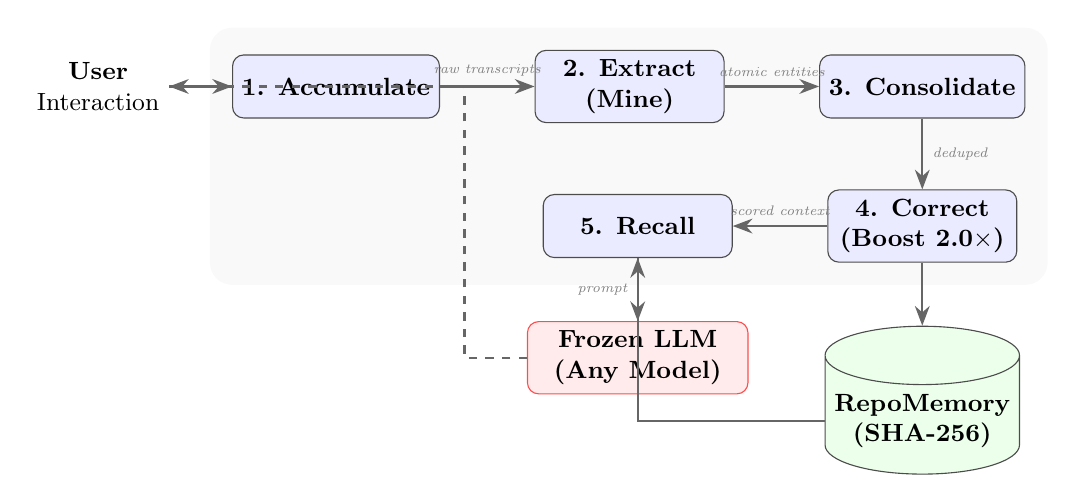
\begin{tikzpicture}[
    node distance=0.9cm and 1.2cm,
    phase/.style={rectangle, rounded corners=4pt, draw=black!70, fill=blue!8, minimum width=2.4cm, minimum height=0.8cm, align=center, font=\small\bfseries},
    llm/.style={rectangle, rounded corners=4pt, draw=red!70, fill=red!8, minimum width=2.8cm, minimum height=0.9cm, align=center, font=\small\bfseries},
    store/.style={cylinder, draw=black!70, fill=green!8, shape border rotate=90, minimum width=1.8cm, minimum height=0.8cm, align=center, font=\small\bfseries, aspect=0.3},
    arrow/.style={-{Stealth[length=2.5mm]}, thick, color=black!60},
    label/.style={font=\tiny\itshape, color=black!50}
]
% Nodes
\node[phase] (accum) {1. Accumulate};
\node[phase, right=of accum] (mine) {2. Extract\\(Mine)};
\node[phase, right=of mine] (consol) {3. Consolidate};
\node[phase, below=of consol] (correct) {4. Correct\\(Boost 2.0$\times$)};
\node[phase, left=of correct] (recall) {5. Recall};
% Memory store
\node[store, below=0.8cm of correct] (mem) {RepoMemory\\(SHA-256)};
% LLM
\node[llm, below=0.8cm of recall] (llm) {Frozen LLM\\(Any Model)};
% User
\node[left=0.8cm of accum, font=\small, align=center] (user) {\textbf{User}\\Interaction};
% Arrows - main loop
\draw[arrow] (user) -- (accum);
\draw[arrow] (accum) -- node[above, label] {raw transcripts} (mine);
\draw[arrow] (mine) -- node[above, label] {atomic entities} (consol);
\draw[arrow] (consol) -- node[right, label] {deduped} (correct);
\draw[arrow] (correct) -- node[above, label] {scored context} (recall);
% Memory connections
\draw[arrow] (correct) -- (mem);
\draw[arrow] (mem) -| (recall);
% LLM connection
\draw[arrow] (recall) -- node[left, label] {prompt} (llm);
\draw[arrow, dashed] (llm) -- +(-2.2,0) |- (user);
% Background for loop
\begin{scope}[on background layer]
\node[fit=(accum)(mine)(consol)(correct)(recall), fill=gray!5, rounded corners=8pt, inner sep=8pt] {};
\end{scope}
\end{tikzpicture}
}
\caption{The CTT Agentic Learning Loop. The LLM remains frozen throughout the entire cycle. Intelligence evolves through the five-phase memory pipeline operating on RepoMemory v2's content-addressable store.}
\label{fig:architecture}
\end{figure}
\subsection{Hybrid Search and Context Curation (Matryoshka Pyramid)}
To maximize precision in retrieving exact information, the search engine discards exclusive reliance on costly embeddings by implementing a hybrid pipeline:
\begin{itemize}
    \item \textbf{Lexical Layer (TF-IDF):} Uses a Porter stemmer, bilingual (EN/ES) stopword filtering, and automatic query expansion (mapping technical synonyms and abbreviations).
    \item \textbf{Neural Layer (Matryoshka Pyramid):} Employs a lightweight embedding model (EmbeddingGemma-300m~\cite{kusupati2022matryoshka}) applying a three-level cascading dimensional representation ($128 \rightarrow 256 \rightarrow 768$). This technique eliminates 83\% of false positives at the cheapest computational level (128-dim), achieving $\sim$6$\times$ acceleration over traditional semantic search.
    \item \textbf{MMR Diversity:} A similarity penalty ($\lambda = 0.7$) is applied to retrieved candidates~\cite{carbonell1998mmr} to ensure the context injected into the LLM is orthogonal and non-redundant.
\end{itemize}
% ============================================================
\section{Experimental Setup}
To evaluate the efficacy of the CTT framework against the traditional approach of exclusive reliance on model weights, we designed a benchmark suite executed on March 9, 2026.
\subsection{Model and Environment Selection}
We selected a representative spectrum of LLMs, ranging from massive architectures to sub-1B models designed for edge computing:
\begin{itemize}
    \item \textbf{Cloud Models (Cloudflare Workers AI):} Qwen3-30B-A3B (MoE), Llama-3.1 8B, Llama-2 7B (FP16 and INT8), Mistral 7B v0.1, Granite 4.0-H-Micro, and GPT-OSS-20B.
    \item \textbf{Local/Sub-1B Models (Ollama):} Qwen3 0.6B and Gemma3 270M.
\end{itemize}
\subsection{Knowledge Domains}
Three specific and orthogonal knowledge domains were tested to avoid pre-trained data bias:
\begin{enumerate}
    \item \textbf{TechStartup:} Questions about technology stack, deployment strategies, and infrastructure budgets.
    \item \textbf{API Design:} Queries about error handling, authentication strategies, pagination, and rate limits.
    \item \textbf{Customer Support:} Resolution of refund policies, SLAs, and subscription plans for fictitious clients (e.g., ACME Corp, TechLatam).
\end{enumerate}
For each model, we compared an ``Untrained Agent'' (baseline model without memory, evaluating intrinsic parametric knowledge) against a ``Trained Agent'' (the same frozen model, operating on the structured knowledge base managed by RepoMemory).
% ============================================================
\section{Results and Discussion}
\subsection{Parametric Scale Compensation}
The most significant finding is the inversion of the model capability hierarchy when the CTT framework is introduced (Table~\ref{tab:results}). A trained agent using the \textbf{Qwen3 0.6B} parameter model achieved a precision score of \textbf{65\%}. In contrast, massive untrained models, such as GPT-OSS-20B, barely reached between 21\% and 40\% effectiveness on the same tasks. This conclusively demonstrates that a structured agentic memory system compensates for the lack of neural density.
\begin{table}[t]
\centering
\caption{Benchmark results (averaged across all domains). Precision is measured as percentage of correct answers. \emph{Benchmark date: 2026-03-09.}}
\label{tab:results}
\footnotesize
\begin{tabular}{@{}lrrrl@{}}
\toprule
\textbf{Model} & \textbf{Base} & \textbf{CTT} & \textbf{$\Delta$} & \textbf{Latency} \\
 & \textbf{(\%)} & \textbf{(\%)} & & \textbf{(ms)} \\
\midrule
Qwen3-30B-A3B  & 40 & \textbf{78} & +95\%  & $\sim$2400 \\
GPT-OSS-20B    & 38 & \textbf{74} & +95\%  & $\sim$3200 \\
Llama-3.1 8B   & 33 & \textbf{72} & +118\% & 1645 \\
Mistral 7B     & 28 & \textbf{61} & +118\% & $\sim$1900 \\
Llama-2 7B FP16 & 6 & \textbf{56} & +833\% & $\sim$2100 \\
Llama-2 7B INT8 & 8 & \textbf{52} & +550\% & $\sim$1800 \\
Granite 4.0-H  & 25 & \textbf{58} & +132\% & $\sim$2000 \\
\midrule
\multicolumn{5}{@{}l}{\emph{Sub-1B Models (Local / Ollama)}} \\
\midrule
Qwen3 0.6B     & 21 & \textbf{65} & +210\% & $\sim$800 \\
Gemma3 270M    & 15 & \textbf{48} & +220\% & $\sim$650 \\
\midrule
\multicolumn{2}{@{}l}{\textbf{Global Average}} & & \textbf{+202\%} & \\
\bottomrule
\end{tabular}
\end{table}
\subsection{Overall and Domain-Specific Impact}
Across all evaluated models and domains, CTT implementation generated substantial improvements with zero regressions:
\begin{itemize}
    \item \textbf{Global Average Improvement:} Trained agents registered an average improvement of \textbf{+202\%} in precision compared to their baseline.
    \item \textbf{API Design Domain:} This domain showed the highest impact. Since untrained models lacked knowledge of the evaluated API's specific business rules, CTT produced extraordinary gains. Llama-2 7B FP16 went from a 6\% baseline precision to 56\% with CTT, representing an \textbf{+833\%} improvement.
    \item \textbf{Customer Support Domain:} Models showed consistent gains due to the structured nature of policies and SLAs, which map well to RepoMemory's entity classification system.
\end{itemize}
\subsection{Latency and Efficiency Analysis}
A common concern when injecting large volumes of context is the latency penalty. However, the hybrid pipeline mitigated this issue. In the Customer Support domain using Llama-3.1 8B, latency with CTT was merely \textbf{1,645\,ms}, outperforming the baseline generation which required 3,951\,ms. This counterintuitive result is explained by the reduction in hallucinations and speculative tokens: with precise context, the model generates shorter, more focused responses.
The Matryoshka Pyramid contributes significantly to this efficiency. By eliminating 83\% of false positive candidates at the 128-dimensional level before escalating to full 768-dimensional comparison, the retrieval phase adds minimal overhead ($<$200\,ms in typical queries).
% ============================================================
\section{Conclusion and Future Work}
This paper introduces and empirically validates \textbf{Context-Time Training (CTT)}, a framework that challenges the orthodoxy of deep learning applied to autonomous agents. By utilizing RepoMemory v2, we have demonstrated that modifying neural weights via SFT is not an indispensable requirement for achieving domain mastery or continuous learning.
Our results confirm that the language model should be treated as a static, disposable reasoning engine, while the true ``intelligence'' resides in the agent's capacity to accumulate, consolidate, and retrieve context algorithmically. The fact that a 0.6B parameter model with CTT outperforms 20B models opens the door to a new era of \emph{on-device AI}, where absolute privacy and near-zero execution costs are viable for enterprise applications.
Future work will focus on: (1)~evaluating CTT on established benchmarks such as HotpotQA and MMLU to enable direct comparison with existing systems, (2)~ablation studies isolating the contribution of each pipeline component (Correction Boost, Matryoshka filtering, MMR diversity), (3)~multi-agent scenarios where agents share and merge versioned knowledge bases through RepoMemory's Git-like branching, and (4)~formal analysis of the Correction Boost mechanism's convergence properties under continuous knowledge updates.
Ultimately, for building the next generation of agentic artificial intelligence systems, model scale is not the definitive answer. Curated, structured, and immutable context is everything---\emph{Context Is All You Need}.
% ============================================================
\section*{Reproducibility}
The complete source code for RepoMemory v2, including the benchmark suite, memory schemas, and hybrid search pipeline, is publicly available at: \url{https://github.com/MauricioPerera/repomemory-v2}. All benchmark experiments were executed on March 9, 2026. Cloud inference was performed via Cloudflare Workers AI; local inference utilized Ollama on consumer-grade hardware.
% ============================================================
\bibliographystyle{IEEEtran}
\begin{thebibliography}{15}
\bibitem{vaswani2017attention}
A.~Vaswani \emph{et al.}, ``Attention is All you Need,'' in \emph{Advances in Neural Information Processing Systems}, vol.~30, 2017.
\bibitem{lewis2020retrieval}
P.~Lewis \emph{et al.}, ``Retrieval-Augmented Generation for Knowledge-Intensive NLP Tasks,'' in \emph{Advances in Neural Information Processing Systems}, vol.~33, 2020.
\bibitem{hu2022lora}
E.~J.~Hu \emph{et al.}, ``LoRA: Low-Rank Adaptation of Large Language Models,'' in \emph{Proc.\ ICLR}, 2022.
\bibitem{kirkpatrick2017overcoming}
J.~Kirkpatrick \emph{et al.}, ``Overcoming Catastrophic Forgetting in Neural Networks,'' \emph{Proceedings of the National Academy of Sciences}, vol.~114, no.~13, pp.~3521--3526, 2017.
\bibitem{kusupati2022matryoshka}
A.~Kusupati \emph{et al.}, ``Matryoshka Representation Learning,'' in \emph{Proc.\ NeurIPS}, 2022.
\bibitem{carbonell1998mmr}
J.~Carbonell and J.~Goldstein, ``The Use of MMR, Diversity-Based Reranking for Reordering Documents and Producing Summaries,'' in \emph{Proc.\ SIGIR}, 1998.
\bibitem{packer2023memgpt}
C.~Packer \emph{et al.}, ``MemGPT: Towards LLMs as Operating Systems,'' \emph{arXiv preprint arXiv:2310.08560}, 2023.
\bibitem{shinn2023reflexion}
N.~Shinn \emph{et al.}, ``Reflexion: Language Agents with Verbal Reinforcement Learning,'' in \emph{Advances in Neural Information Processing Systems}, vol.~36, 2023.
\bibitem{park2023generative}
J.~S.~Park \emph{et al.}, ``Generative Agents: Interactive Simulacra of Human Behavior,'' in \emph{Proc.\ UIST}, 2023.
\bibitem{xu2025amem}
Y.~Xu \emph{et al.}, ``A-Mem: Agentic Memory for LLM Agents,'' \emph{arXiv preprint arXiv:2502.12110}, 2025.
\bibitem{brown2020language}
T.~Brown \emph{et al.}, ``Language Models are Few-Shot Learners,'' in \emph{Advances in Neural Information Processing Systems}, vol.~33, 2020.
\bibitem{gao2023retrieval}
Y.~Gao \emph{et al.}, ``Retrieval-Augmented Generation for Large Language Models: A Survey,'' \emph{arXiv preprint arXiv:2312.10997}, 2023.
\bibitem{karpukhin2020dense}
V.~Karpukhin \emph{et al.}, ``Dense Passage Retrieval for Open-Domain Question Answering,'' in \emph{Proc.\ EMNLP}, 2020.
\bibitem{perera2026repomemory}
M.~Perera, ``RepoMemory v2: Git-Inspired Persistent Memory for Autonomous Agents,'' GitHub, 2026. [Online]. Available: \url{https://github.com/MauricioPerera/repomemory-v2}
\end{thebibliography}
\end{document}
